\documentclass[10pt]{article}
\usepackage[T1]{fontenc}
\usepackage[utf8]{inputenc}
\usepackage[main=portuguese,provide=*]{babel} % para indice em português
\usepackage{url}
\usepackage{graphicx}
\usepackage{caption}
\usepackage{tikz}
\usetikzlibrary{arrows.meta, positioning}
\usepackage[margin=1in]{geometry}

% or customize, for example:
% \usepackage[left=1in,right=1in,top=0.8in,bottom=0.8in]{geometry}
\graphicspath{ {./figures/} }

\newcommand{\imageplaceholder}[2]{%
  \fbox{%
    \parbox[c][#2][c]{0.92\linewidth}{\centering #1}%
  }%
}


\begin{document}

\setcounter{tocdepth}{3}

\begin{titlepage}
	\begin{center}
		\vspace*{1cm}

		
    {\fontsize{17}{16}\selectfont \textbf{Análise e gestão de horários IV}}
     
		
		\vspace{0.5cm}
		U.Porto - L.EIC - Projeto Integrador\\
		
		\vspace{1.5cm}

        \textbf{Ana Silva - up202308786}\\ 
		\textbf{Claudio Meireles - up202306618}\\
		\textbf{Diogo Faria - up202205982}\\ 
		\textbf{Pedro Coelho - up202306714}\\ 
		
				\vfill
		
		\includegraphics[width=0.4\textwidth]{UPORTO_fundotransparente}
		
		\vfill
		
	
		
		Licenciatura em Engenharia Informática e Computação
		
		\vspace{0.8cm}
		
		
		\textbf{Supervisor U.Porto}: Professor Daniel Castro Silva\\

\vspace{0.4cm}
		5 de julho de 2026
		
	\end{center}
\end{titlepage}


\thispagestyle{empty} 
\clearpage

\thispagestyle{empty}
\tableofcontents

 \clearpage
 
\section{Introdução}

    O presente relatório descreve o trabalho realizado no âmbito do Projeto Integrador, centrado no desenvolvimento contínuo de uma plataforma de apoio à gestão de horários académicos na FEUP. Ao longo do documento apresenta-se a natureza do problema tratado, o contexto em que o projeto se insere, as decisões tomadas durante o desenvolvimento e uma avaliação dos resultados obtidos.
	
	\subsection{Enquadramento}

    Organizar horários que satisfaçam simultaneamente as exigências de todas as partes envolvidas é uma dificuldade concreta: é preciso acomodar salas com capacidade limitada, respeitar a disponibilidade de cada docente, impedir que aulas da mesma turma colidam e, ao mesmo tempo, garantir que a carga semanal dos alunos fica distribuída de forma razoável. Cada um destes fatores restringe o espaço de soluções possíveis, e é a interação entre todos eles que torna a tarefa tão exigente.\\
    \\
    Na Faculdade de Engenharia da Universidade do Porto, os horários são preparados a cada semestre segundo um fluxo que combina automatismo e intervenção humana.\\
    Numa primeira fase, uma aplicação especializada produz uma versão preliminar dos horários a partir das restrições de salas e docentes.\\
    Cabe depois às comissões de horários de cada curso rever essa versão: confirmam que as regras foram cumpridas, procuram tirar melhor partido das salas disponíveis e reorganizam as aulas de modo a compactar os horários individuais dos docentes.\\
    Este ciclo de revisão pode repetir-se até se atingir um resultado considerado satisfatório. Só então as alterações seguem para a equipa de sistemas de informação, que as consolida e publica a versão definitiva.\\
    \\
    O problema é que a fase intermédia - \emph{a revisão manual} - consome muito tempo e está sujeita a lapsos. As soluções geradas automaticamente tendem a ficar aquém do ideal, deixando às comissões o encargo de corrigir desequilíbrios na distribuição do serviço docente e de equilibrar a carga horária dos alunos. Como esse trabalho exige cruzar mentalmente turmas, docentes, salas e compatibilidades de horário, detetar conflitos torna-se particularmente complicado.
    \\
    É precisamente sobre esta fase que o projeto procura atuar. A ideia de uma ferramenta que apoie a revisão de horários e a deteção de conflitos não é nova: edições anteriores do Projeto Integrador~\cite{carvalho2023, correia2024, oliveira2025} deram origem a uma plataforma que permite visualizar horários e realizar trocas de forma mais rápida e intuitiva do que as folhas de cálculo tradicionalmente usadas para o efeito. Em 2024, num registo complementar, Miguel Lopes desenvolveu na sua dissertação de M.EIC~\cite{lopes2024} um otimizador automático de horários, abrindo caminho para conjugar o ganho de eficiência da automatização com o controlo que só a edição manual oferece. Partindo do princípio de que os ajustes manuais nunca deixarão de ser necessários, faz sentido continuar a investir numa ferramenta desenhada especificamente para essa tarefa - algo que, enquanto estudantes da FEUP, encarámos com interesse acrescido, por nos tocar diretamente.


	\subsection{Objetivos e resultados esperados}
    \label{sec:objetivos}

    O presente projeto teve como objetivo geral dar continuidade ao desenvolvimento da aplicação web de análise e gestão de horários criada em edições anteriores do Projeto Integrador, procurando transformá-la numa solução mais eficiente e fiável, e mais fácil de manter e evoluir.
    Para concretizar este objetivo, pretendeu-se otimizar o processo de ingestão e processamento dos horários publicados pela FEUP, reduzindo o respetivo tempo de execução sem comprometer a integridade e a completude dos dados. Pretendeu-se também reformular a interface e a experiência de utilização do editor de horários, tornando a visualização, filtragem e edição das aulas mais claras, rápidas e responsivas.\\
    \\
    Adicionalmente, foram definidos como objetivos a conclusão da funcionalidade de seleção e persistência de grupos de aulas em paralelo, o reforço da deteção de conflitos associados a salas, docentes e turmas e o desenvolvimento de uma página de exportação mais completa, capaz de comparar os horários original e editado, identificar alterações e conflitos e apresentar um plano de modificações devidamente organizado.
    Outro objetivo relevante consistiu em aumentar a fiabilidade e a manutenibilidade da aplicação. Para esse efeito, pretendeu-se reduzir a dependência de código legado, melhorar a separação entre a interface, a lógica de negócio e o acesso aos dados, introduzir modelos de dados mais estruturados e adotar ferramentas de validação, testes automáticos, análise estática de código e documentação detalhada do projeto. Estas alterações procuraram diminuir a probabilidade de regressões, facilitar a deteção de erros e tornar a aplicação mais simples de compreender, testar e evoluir por equipas futuras.\\
    \\
    Como resultados esperados, pretendia-se obter uma redução significativa dos tempos de processamento, uma interação mais rápida e intuitiva com os horários, uma deteção de conflitos mais consistente e explicável, uma exportação das alterações mais clara e completa e uma base de código mais robusta, modular, testável e preparada para desenvolvimentos futuros.

    
	\subsection{Estrutura do relatório}
	
	A primeira secção, Metodologia utilizada e principais atividades desenvolvidas, descreve a metodologia de trabalho adotada, os recursos e ferramentas utilizados, os principais intervenientes no projeto e as respetivas responsabilidades. Apresenta também a distribuição temporal das atividades realizadas e os principais momentos do desenvolvimento.\\
    \\
    A segunda secção, Desenvolvimento da solução, apresenta o problema abordado, os requisitos funcionais e não funcionais e as principais restrições identificadas. Nesta secção são ainda descritas a arquitetura da aplicação, as tecnologias utilizadas e as decisões técnicas tomadas. Posteriormente, é apresentado o trabalho desenvolvido nas diferentes componentes do sistema, nomeadamente a otimização do processo de ingestão e processamento dos horários, a reformulação da interface e do editor, a seleção de aulas em paralelo, a deteção de conflitos e a exportação das alterações. São também descritas as medidas adotadas para melhorar a fiabilidade, a testabilidade e a manutenibilidade da aplicação, bem como os métodos utilizados para validar a solução e os resultados obtidos.\\
    \\
    Por fim, a secção Conclusões sintetiza os principais resultados alcançados e relaciona-os com os objetivos inicialmente definidos. Inclui ainda as contribuições individuais dos elementos da equipa, as principais lições aprendidas, as limitações do trabalho desenvolvido e possíveis direções para trabalho futuro.


\section{Metodologia utilizada e principais atividades desenvolvidas}

\subsection{Metodologia utilizada}

    A equipa adotou um processo de desenvolvimento iterativo e incremental~\cite{despa2014comparative}, organizado em torno do repositório GitHub~\cite{github} do projeto e de reuniões de acompanhamento praticamente semanais com o supervisor.
    O fluxo de trabalho seguiu o modelo \emph{GitHub Flow}: cada funcionalidade ou correção foi desenvolvida numa \emph{branch} própria, com uma convenção de nomes por área (\texttt{backend/*}, \texttt{frontend/*}), e integrada na \emph{branch} de integração \texttt{dev} através de \emph{pull requests} sujeitos a revisão de código por outro elemento da equipa. Ao longo do projeto foram integrados mais de 230 \emph{pull requests}, num total de cerca de 960 \emph{commits}. A \emph{branch} \texttt{main} preservou a versão da aplicação herdada das edições anteriores, servindo de referência estável para medir a evolução do trabalho.\\
    \\
    A qualidade do código foi assegurada de forma automática em todos os \emph{pull requests} através de \emph{pipelines} de integração contínua (GitHub Actions): no \emph{backend}, \emph{linting} e formatação com ruff e execução dos testes com pytest; no \emph{frontend}, \emph{linting} (ESLint), formatação (Prettier), verificação de tipos (TypeScript) e testes (Vitest). Estas verificações são reforçadas por \emph{hooks} de \texttt{pre-commit} locais e pela verificação de tipos do \emph{backend} em modo estrito (Pyright), realizada em ambiente de desenvolvimento. A atualização de dependências foi automatizada com o Dependabot, em ciclo semanal, garantindo que a aplicação se manteve alinhada com as versões mais recentes das bibliotecas utilizadas. Os ambientes de desenvolvimento e produção foram uniformizados com Docker e \texttt{docker-compose}, orquestrados por um \texttt{Makefile}, e a gestão de dependências Python migrou de pipenv para uv. Para permitir desenvolver e testar a ingestão sem depender do sítio institucional, foi criado um \emph{mirror} local das páginas de horários.
	
	
\subsection{Intervenientes, papéis e responsabilidades}

    O projeto foi desenvolvido por uma equipa de quatro estudantes da L.EIC, com supervisão do Professor Daniel Castro Silva (U.Porto), o que garantiu à equipa acesso contínuo à perspetiva dos utilizadores finais da ferramenta. São ainda partes interessadas as comissões de horários dos cursos da FEUP, destinatárias finais da ferramenta, e as equipas de edições anteriores do Projeto Integrador, cujo trabalho serviu de ponto de partida.
    \\\\
    %% NOTA: distribuição inferida do histórico do repositório (git) — confirmar/ajustar, sobretudo a repartição das aulas em paralelo entre o backend (Cláudio) e o frontend (Pedro).
    Dentro da equipa, as responsabilidades principais distribuíram-se da seguinte forma:
    \textbf{Ana Silva} - protótipo do editor de horários no \emph{frontend} (grelha semanal, painéis de edição e de conflitos, barra de navegação e filtros) e páginas de autenticação;
    \textbf{Cláudio Meireles} - reestruturação e reescrita do \emph{backend}: o \emph{pipeline} de ingestão e processamento dos horários e a respetiva otimização, o novo modelo de dados (SQLAlchemy e camada de DAOs) e a API do projeto;
    \textbf{Diogo Faria} - módulo de exportação: comparação entre o horário original e o editado, deteção de conflitos na exportação e cálculo do plano de modificações por análise de dependências, bem como a respetiva página;
    \textbf{Pedro Coelho} - desenvolvimento da funcionalidade de aulas em paralelo, desde a deteção até à criação do protótipo da página de seleção; implementação da gestão de conflitos, incluindo a deteção, a pré-deteção (em caso de alteração de uma aula) e a interface do painel de conflitos; e primeira integração com o otimizador.

\subsection{Atividades desenvolvidas}

    %% TODO: complementar com diagrama de Gantt~\cite{gantt} e acrescentar
    %% eventos relevantes (apresentações intermédias, demos ao supervisor).

    O trabalho decorreu entre fevereiro e julho de 2026. A Tabela~\ref{tab:atividades} resume as principais fases e entregas.
 
\begin{table}[h]
\centering
\footnotesize
\begin{tabular}{@{}p{2.2cm} p{11.2cm}@{}}
\hline
\textbf{Período} & \textbf{Atividades principais} \\
\hline
Fevereiro &
Análise da base de código herdada; limpeza e reorganização; introdução de \emph{linter} e formatador (ruff) com \texttt{pre-commit}; correção de \emph{bugs} e de vulnerabilidades no \emph{parser} existente. \\
Março &
Novo modelo de dados (SQLAlchemy, camada de DAOs, base SQLite por projeto); novo pipeline de ingestão (\emph{scraper} e \emph{parsers} das páginas de horários); reestruturação do repositório em \texttt{backend/} e \texttt{frontend/}; arranque da SPA em React (autenticação, gestão de projetos, \emph{dashboard}); integração contínua; Docker; \emph{mirror} local do sítio institucional. \\
Abril &
Endpoints de dados do projeto (cursos, anos, UCs, turmas, sessões, docentes, salas, estatísticas); páginas de detalhe do \emph{dashboard}; protótipo do editor de horários; deteção de blocos paralelos no \emph{backend}; migração para uv. \\
Maio &
Consolidação do editor de horários (filtros, vistas partilháveis por URL, acessibilidade, testes); remoção do código legado (templates e ficheiros estáticos Django); refatoração e otimização da API. \\
Junho--julho &
Relação UC--ano muitos-para-muitos; indisponibilidades nas páginas de detalhe; testes de \emph{frontend} na integração contínua; documentação de arquitetura; desenvolvimento da deteção de conflitos integrada no editor, da seleção de aulas em paralelo com visualização em grafo e do módulo de exportação; elaboração do relatório final. \\
\hline
\end{tabular}
\caption{Fases do projeto e atividades principais.}
\label{tab:atividades}
\end{table} 


\section{Desenvolvimento da solução}

\subsection{Requisitos}

    Os requisitos desta edição resultam de três fontes principais: o estado da plataforma herdada das edições anteriores e as limitações aí identificadas; as prioridades definidas com o supervisor no arranque do projeto; e as restrições impostas pelo próprio contexto institucional, nomeadamente o formato das páginas de horários publicadas no SIGARRA.
    \\\\
    Em termos funcionais, a aplicação deve: ingerir automaticamente os horários publicados pela FEUP, incluindo cursos, anos, unidades curriculares, turmas, sessões, docentes, salas e respetivas indisponibilidades (\emph{red blocks}); suportar múltiplos projetos de edição, cada um com os seus dados isolados e com uma cópia do estado original para posterior comparação; disponibilizar uma área de consulta (\emph{dashboard}) com listas e páginas de detalhe das várias entidades, incluindo o horário semanal de cada uma; oferecer um editor visual de horários com filtragem por curso, ano, unidade curricular, turma, dia e docente, e com edição das sessões (docente, sala, turma, dia e hora); permitir identificar e confirmar grupos de aulas lecionadas em paralelo; detetar conflitos de docentes, salas e turmas, incluindo violações de indisponibilidades, distinguindo os conflitos herdados do horário original dos introduzidos pela edição; e exportar as alterações efetuadas sob a forma de um plano de modificações ordenado e aplicável.
    \\\\
    Quanto a requisitos não funcionais, destacam-se: o desempenho, tanto na ingestão (processar um curso completo em tempo aceitável) como na interface (manter a interação fluida com centenas de sessões e tabelas com muitas linhas); a usabilidade e a acessibilidade, incluindo navegação por teclado, semântica adequada para leitores de ecrã e respeito pelas preferências de movimento reduzido; a fiabilidade e manutenibilidade da base de código, através de tipagem estática de ponta a ponta, testes automáticos e documentação; e a facilidade de instalação e implantação, com ambientes reprodutíveis.
    \\\\
    O projeto esteve ainda sujeito a restrições relevantes: a obtenção dos dados depende de \emph{web scraping} das páginas do SIGARRA, cuja estrutura não é controlada pela equipa; a aplicação não escreve de volta no sistema institucional, pelo que o resultado final da edição é um plano de alterações a aplicar pelos serviços competentes; e o calendário académico do Projeto Integrador limitou o âmbito ao conjunto de funcionalidades priorizadas com o supervisor.


\subsection{Arquitetura e tecnologias}

    A aplicação está organizada em dois módulos principais: um \emph{backend} em Python/Django, que expõe uma API JSON sob \texttt{/api/}, e um \emph{frontend} em React/TypeScript, uma aplicação de página única (SPA) que serve todas as páginas visíveis ao utilizador. Em produção, o Django serve também o \emph{frontend} compilado, ficando toda a navegação do lado do cliente a cargo do React Router.
    \\\\
    A versão herdada era um monólito Django com páginas geradas no servidor - um único ficheiro de vistas com cerca de 1\,800 linhas - com acesso a dados por SQL manual, sem testes nem integração contínua. A opção por uma separação API/SPA justificou-se por três razões: permitir que os elementos da equipa trabalhassem em paralelo sobre contratos de API bem definidos; introduzir tipagem de ponta a ponta (Pydantic na validação de pedidos e respostas do \emph{backend}, TypeScript estrito no \emph{frontend}), reduzindo classes inteiras de erros; e melhorar a experiência de utilização, uma vez que a edição interativa de horários exige atualizações de interface imediatas, difíceis de conseguir com páginas renderizadas no servidor. Esta reestruturação implicou a migração integral das páginas existentes e a remoção do código legado correspondente, num saldo global, face à versão herdada, de 779 ficheiros alterados ($+54\,723$/$-54\,998$ linhas).
    \\\\
    \textbf{Persistência.} O \emph{backend} usa duas camadas de base de dados distintas. Uma meta-base de dados única (SQLite, gerida pelo ORM do Django) guarda as contas de utilizador e os metadados de cada projeto. Os dados de horários de cada projeto vivem numa base SQLite \emph{própria}, definida com modelos SQLAlchemy e acedida através de uma camada de \emph{Data Access Objects} (DAOs) partilhada pela ingestão e pela API. Cada projeto mantém dois ficheiros: a base de trabalho (\texttt{general\_database}), lida e editada pela API, e um \emph{snapshot} tirado no fim da ingestão (\texttt{initial\_database}), que preserva o horário original e serve de referência à deteção de conflitos pré-existentes e ao módulo de exportação (Secção~\ref{sec:exporter}). Este isolamento por projeto simplifica a criação e eliminação de cenários alternativos de edição e elimina interferências entre projetos.
    \\\\
    \textbf{Ingestão.} A ingestão é um pacote Python independente das \emph{apps} Django, composto por um \emph{scraper} (\texttt{requests} + BeautifulSoup) e por \emph{parsers} dedicados a cada tipo de página (menus de curso, páginas de turma, páginas de docente, blocos de indisponibilidade e salas), que validam os dados extraídos com estruturas tipadas e verificações explícitas antes de os persistirem através dos DAOs.
    \\\\
    \textbf{Frontend.} A SPA usa Vite como servidor de desenvolvimento e empacotador, TanStack Query para o estado do servidor (\emph{cache} e mutações), React Router para navegação, Tailwind CSS para estilos e TanStack Virtual para virtualização de tabelas grandes. Não existe biblioteca de estado global: o estado de interface vive em \emph{hooks} e no URL, o que torna as vistas do editor partilháveis por ligação. A lógica não trivial do editor está isolada em \emph{hooks} e funções puras com testes unitários (Vitest).

\begin{center}
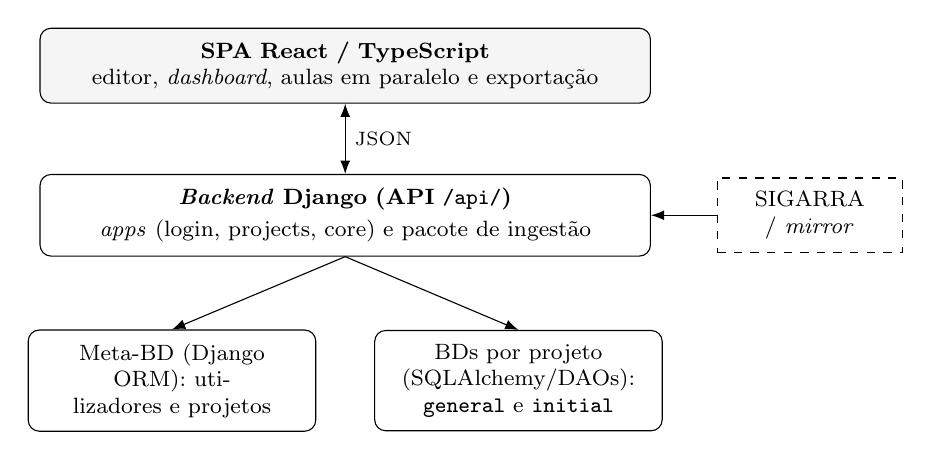
\begin{tikzpicture}[
  >=Latex, font=\footnotesize,
  comp/.style={rectangle, rounded corners, draw, align=center, inner sep=5pt},
  ext/.style={rectangle, draw, dashed, align=center, inner sep=5pt}
]
  \node[comp, fill=black!4, text width=7.4cm] (spa) at (0,0) {\textbf{SPA React / TypeScript}\\ editor, \emph{dashboard}, aulas em paralelo e exportação};
  \node[comp, text width=7.4cm] (backend) at (0,-1.9) {\textbf{\emph{Backend} Django (API \texttt{/api/})}\\[2pt] \emph{apps} (login, projects, core) e pacote de ingestão};
  \node[ext, text width=2cm] (sig) at (5.9,-1.9) {SIGARRA / \emph{mirror}};
  \node[comp, text width=3.3cm] (meta) at (-2.2,-4.0) {Meta-BD (Django ORM): utilizadores e projetos};
  \node[comp, text width=3.3cm] (proj) at (2.2,-4.0) {BDs por projeto (SQLAlchemy/DAOs): \texttt{general} e \texttt{initial}};
  \draw[<->] (spa) -- node[right, font=\scriptsize] {JSON} (backend);
  \draw[->] (sig) -- (backend);
  \draw[->] (backend.south) -- (meta.north);
  \draw[->] (backend.south) -- (proj.north);
\end{tikzpicture}
\captionof{figure}{Arquitetura geral da aplicação.}
\label{fig:arquitetura}
\end{center}

    \textbf{Dificuldades técnicas e resolução.}  A primeira grande dificuldade foi o desempenho da ingestão: a versão inicial fazia um pedido à base de dados por cada entidade inserida, o que tornava o processo demorado. A solução passou por inserções em lote, \emph{caches} de consultas durante a ingestão e controlo explícito do \emph{flush} das sessões SQLAlchemy.
    Outro problema foi a fragilidade do \emph{scraping}: para desenvolver e testar sem depender do sítio institucional (e sem o sobrecarregar), foi criado um \emph{mirror} local das páginas de horários, usado como fonte de dados em desenvolvimento.
    Já no editor, o desafio foi manter a interface fluida com centenas de sessões em ecrã, o que obrigou a virtualização de listas, memoização e extração de lógica para funções puras, além de otimizações nas consultas da API (índices nas tabelas de junção, \emph{eager loading} das relações e eliminação de \emph{joins} redundantes).
    Por último, a deteção de blocos em paralelo deu mais trabalho do que o esperado: a abordagem inicial, baseada em \emph{self-joins} de sessões, revelou-se lenta, e acabou substituída por uma modelação em grafo, em que os grupos candidatos são componentes ligados de um grafo de sobreposição de semanas, com as arestas construídas por agrupamento de \emph{slots}.
    \\\\
    As tecnologias utilizadas resumem-se na Tabela~\ref{tab:tecnologias}.
 
\begin{table}[h]
\centering
\footnotesize
\begin{tabular}{@{}p{2.6cm} p{10.8cm}@{}}
\hline
\textbf{Componente} & \textbf{Tecnologias} \\
\hline
Backend & Python, Django 6 (Daphne/ASGI, WhiteNoise), SQLAlchemy 2, Pydantic 2, requests + BeautifulSoup 4 \\
Frontend & React 19, TypeScript 6 (estrito), Vite 8, React Router 7, TanStack Query 5, TanStack Virtual 3, Tailwind CSS 4 \\
Qualidade & Ruff, Pyright, ESLint, Prettier, Vitest, pre-commit \\
Infraestrutura & Docker + docker-compose, Makefile, uv, GitHub Actions (CI), Dependabot \\
\hline
\end{tabular}
\caption{Tecnologias utilizadas por componente.}
\label{tab:tecnologias}
\end{table}
 

\subsection{Solução desenvolvida}

Esta secção apresenta a solução na ótica do utilizador, seguindo o fluxo típico de utilização: criação de um projeto e ingestão dos horários, consulta no \emph{dashboard}, edição no editor de horários, confirmação de aulas em paralelo, análise de conflitos e, por fim, exportação das alterações.

\subsubsection{Visão geral e gestão de projetos}
\label{sec:overview}

    O acesso à aplicação é feito por autenticação com conta própria, existindo fluxos de recuperação e alteração de palavra-passe. Depois de autenticado, o utilizador chega à página inicial, que lista os seus projetos sob a forma de cartões, com o estado de cada um visível de imediato - em ingestão, pronto a usar ou com falha na ingestão.
    \\\\
    Um \emph{projeto} é a unidade central da aplicação: representa um cenário de edição independente, com uma cópia própria dos dados de horários. Para criar um projeto basta indicar um nome e o endereço da página de horários a ingerir; a ingestão decorre em segundo plano e, quando termina, é guardado um \emph{snapshot} do estado original, que servirá mais tarde de referência à deteção de conflitos pré-existentes e à exportação. Os projetos podem ser renomeados e eliminados, e o isolamento dos dados por projeto permite explorar cenários alternativos de edição sem qualquer interferência entre eles.
    
\begin{center}
\begin{minipage}[t]{0.48\textwidth}
  \centering
  \includegraphics[width=1.0\textwidth]{figures/home_page.png}
  \captionof{figure}{Página inicial com a lista de projetos e o respetivo estado.}
  \label{fig:home}
\end{minipage}\hfill
\begin{minipage}[t]{0.48\textwidth}
  \centering
  \includegraphics[width=1.0\textwidth]{figures/novo_projeto.png}
  \captionof{figure}{Criação de um novo projeto.}
  \label{fig:new-project}
\end{minipage}
\end{center}

\subsubsection{Ingestão e processamento de dados}
\label{sec:ingestion}

    A ingestão é o processo que dá vida a um projeto: percorre as páginas de horários publicadas pela FEUP e delas extrai, para a base de dados do projeto, os cursos, anos, unidades curriculares, turmas, sessões, docentes e salas, bem como os períodos de indisponibilidade de cada recurso (\emph{blocos vermelhos}). Todo este trabalho está reunido num pacote Python autónomo, independente das \emph{apps} Django, orquestrado por um gestor de ingestão que corre numa \emph{thread} em segundo plano - a criação de um projeto responde de imediato e o estado da ingestão (em curso, concluída ou falhada) é registado e refletido na página inicial. A título de ordem de grandeza, o conjunto de páginas usado em desenvolvimento cobre 51 cursos, 661 docentes e 149 salas, dando origem a dezenas de milhares de sessões.
    \\\\
    \textbf{Fases do \emph{pipeline}.} A ingestão está organizada como uma sequência de fases (Figura~\ref{fig:ingestion}). Começa pela leitura do menu de navegação do sítio, de onde o \emph{scraper} (\texttt{requests} + BeautifulSoup) extrai três estruturas: a lista de docentes, a hierarquia curso\,$\rightarrow$\,ano\,$\rightarrow$\,turma com as ligações para as páginas semanais, e a lista de salas. Antes de qualquer escrita na base de dados, são descarregadas todas as páginas semanais das turmas, ficando o seu conteúdo já convertido em memória; concentrar assim o acesso à rede evita intercalar pedidos HTTP com operações de base de dados. Só depois começa a persistência, fase a fase: os docentes e as suas indisponibilidades; a hierarquia de cursos, anos e turmas; as salas; e, por fim, as sessões, que constituem o grosso dos dados. Duas fases de pós-processamento completam o resultado - a atribuição de turnos às turmas, calculada a partir das aulas teóricas (informação que não consta diretamente das páginas), e a reconstrução dos identificadores de bloco descrita adiante. No final, a base de dados de trabalho é copiada para um \emph{snapshot} imutável, que preserva o horário original e serve de referência à deteção de conflitos pré-existentes e à exportação.

\begin{center}
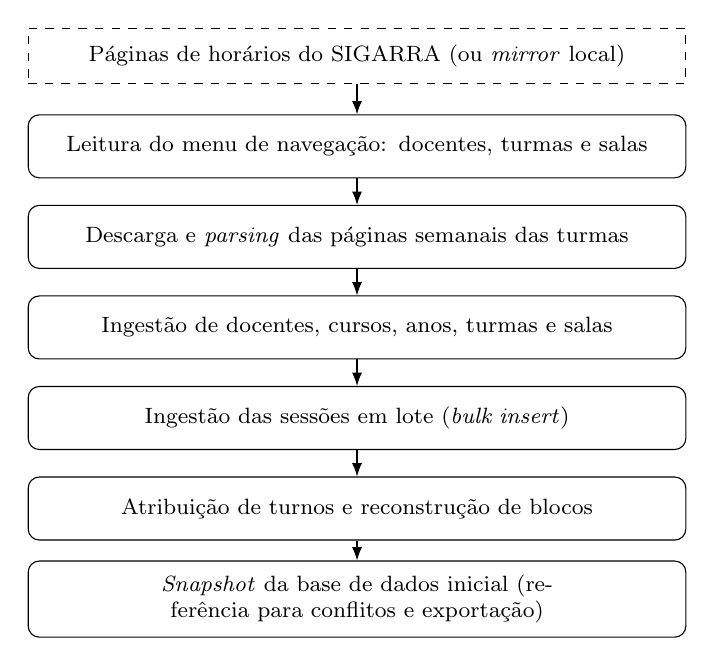
\begin{tikzpicture}[
  >=Latex, font=\footnotesize,
  box/.style={rectangle, rounded corners, draw, align=center, text width=8cm, inner sep=5pt, minimum height=8mm},
  src/.style={rectangle, draw, dashed, align=center, text width=8cm, inner sep=5pt, minimum height=7mm}
]
  \node[src] (n0) at (0,0) {Páginas de horários do SIGARRA (ou \emph{mirror} local)};
  \node[box] (n1) at (0,-1.15) {Leitura do menu de navegação: docentes, turmas e salas};
  \node[box] (n2) at (0,-2.30) {Descarga e \emph{parsing} das páginas semanais das turmas};
  \node[box] (n3) at (0,-3.45) {Ingestão de docentes, cursos, anos, turmas e salas};
  \node[box] (n4) at (0,-4.60) {Ingestão das sessões em lote (\emph{bulk insert})};
  \node[box] (n5) at (0,-5.75) {Atribuição de turnos e reconstrução de blocos};
  \node[box] (n6) at (0,-6.90) {\emph{Snapshot} da base de dados inicial (referência para conflitos e exportação)};
  \draw[->] (n0) -- (n1);
  \draw[->] (n1) -- (n2);
  \draw[->] (n2) -- (n3);
  \draw[->] (n3) -- (n4);
  \draw[->] (n4) -- (n5);
  \draw[->] (n5) -- (n6);
\end{tikzpicture}
\captionof{figure}{Fases do \emph{pipeline} de ingestão de horários.}
\label{fig:ingestion}
\end{center}

    \textbf{Extração e validação.} Cada tipo de página tem um \emph{parser} dedicado. Como o horário é apresentado em tabelas HTML, os \emph{parsers} reconstroem primeiro a matriz de células - respeitando as junções de linhas e colunas - e só depois dela derivam as sessões, com os respetivos tempos, tipologias, docentes e salas. Os dados extraídos são representados por estruturas tipadas e sujeitos a verificações explícitas em cada \emph{parser} (contagens de tabelas e de células, expressões regulares sobre as siglas, datas bem formadas, tipologias reconhecidas): qualquer desvio ao formato esperado interrompe a ingestão com um erro claro, em vez de gerar dados corrompidos de forma silenciosa. Este rigor é indispensável porque a estrutura das páginas não é controlada pela equipa e pode mudar sem aviso. Vários casos-limite reais são tratados de forma dedicada: sessões partilhadas por mais do que uma unidade curricular, aulas que decorrem apenas em parte do semestre (expandidas para uma ocorrência por semana), aulas sem sala física (assinaladas como \emph{online}), docentes sem indisponibilidades (que não têm ligação no menu e são recuperados a partir das páginas das turmas) e salas não catalogadas (registadas como desconhecidas).
    \\\\
    \textbf{Reconstrução de blocos.} O sítio institucional divide o horário de cada turma em várias páginas por intervalo de datas, pelo que uma mesma aula recorrente surge fragmentada em vários registos independentes. Para reconstruir a noção de \emph{bloco} - uma aula que se repete, igual, ao longo de várias semanas -, cada sessão é caracterizada por uma assinatura invariante na semana (dia, hora de início, duração, tipologia, conjunto de docentes, conjunto de salas e os pares turma--UC), e todas as sessões com a mesma assinatura são reunidas sob um identificador de bloco comum. Esta reconstrução é a base das funcionalidades que raciocinam sobre aulas inteiras, como a deteção de aulas em paralelo (Secção~\ref{sec:parallel}) e a exportação (Secção~\ref{sec:exporter}).
    \\\\
    \textbf{Desempenho.} A redução do tempo de ingestão foi um dos objetivos centrais desta edição - a ingestão foi, de resto, uma preocupação de desempenho recorrente nas edições anteriores~\cite{carvalho2023, correia2024}. A versão herdada por esta equipa escrevia cada entidade na base de dados com uma operação individual, emitindo um pedido por cada registo inserido, o que domina o tempo total quando se persistem dezenas de milhares de sessões: uma ingestão completa demorava mais de 12 minutos. A reescrita atacou o problema em três frentes: (i) as escritas deixaram de sincronizar com a base de dados a cada registo, passando a ser acumuladas em memória e enviadas em lote uma vez por tipo de entidade; (ii) as sessões e as suas associações - as tabelas de maior dimensão - são inseridas com operações \emph{bulk} únicas, gerando-se os identificadores em Python para dispensar idas à base de dados; e (iii) as chaves estrangeiras (docentes, turmas, salas, UCs) são resolvidas a partir de \emph{caches} em memória construídas durante a própria ingestão, eliminando as consultas de pesquisa que antes acompanhavam cada inserção. Com estas mudanças, o número de acessos à base de dados deixou de ser proporcional ao número de entidades para passar a depender apenas do número de \emph{tipos} de entidade, e o tempo de uma ingestão completa passou de mais de 12 minutos para cerca de 2 minutos - dos quais a quase totalidade corresponde já ao tempo de descarregar as páginas do servidor institucional, e não ao processamento ou à persistência dos dados.
    \\\\
    \textbf{Ambiente reprodutível.} Depender do sítio institucional para desenvolver e testar a ingestão é frágil e indesejável, tanto pela variabilidade do acesso como por não ser aceitável sobrecarregá-lo com pedidos repetidos. Criou-se, por isso, um \emph{mirror} local das páginas de horários, servido por um contentor Docker próprio, que funciona como fonte de dados controlada e reprodutível durante o desenvolvimento. A partir desse \emph{mirror} foram ainda capturadas páginas reais, guardadas comprimidas no repositório, que alimentam testes automáticos dos \emph{parsers}: além de verificarem a coerência da extração, funcionam como alarme sempre que o formato das páginas do SIGARRA muda.

\subsubsection{Dashboard de consulta}
\label{sec:dashboard}

    Depois de a ingestão terminar, o \emph{dashboard} do projeto reúne num único espaço informação que no sistema institucional está dispersa por dezenas de páginas. A vista principal organiza-se em separadores - cursos, anos, unidades curriculares, turmas, docentes e salas - com cartões de estatísticas globais e tabelas pesquisáveis. As tabelas usam virtualização de linhas, pelo que listas com centenas de entradas (por exemplo, todos os docentes de um curso) permanecem fluidas.
    \\\\
    Cada linha dá acesso a uma página de detalhe. A página de um docente, por exemplo, mostra as suas estatísticas, o horário semanal completo e os períodos de indisponibilidade (\emph{red blocks}); as páginas de salas, turmas e unidades curriculares seguem o mesmo padrão, e a página de um curso lista as UCs e turmas de cada ano. Os horários apresentados nestas páginas usam a mesma grelha semanal do editor, com as sessões clicáveis para consultar detalhes e navegar entre entidades relacionadas - por exemplo, da sessão para a página da UC ou da turma. Sessões lecionadas apenas em parte do semestre apresentam o intervalo de semanas correspondente.
    
\begin{center}
\begin{minipage}[t]{0.48\textwidth}
  \centering
  \includegraphics[width=1.0\textwidth]{figures/dashboard.png}
  \captionof{figure}{Vista principal do \emph{dashboard}, com estatísticas globais e tabelas pesquisáveis.}
  \label{fig:dashboard}
\end{minipage}\hfill
\begin{minipage}[t]{0.48\textwidth}
  \centering
  \includegraphics[width=1.0\textwidth]{figures/docente_detalhe.png}
  \captionof{figure}{Página de detalhe de um docente, com o horário semanal e as indisponibilidades.}
  \label{fig:detail-page}
\end{minipage}
\end{center}

\subsubsection{Editor de horários}
\label{sec:editor}

    O editor de horários, componente central da aplicação, apresenta uma grelha semanal em que cada dia se subdivide em colunas por turma - redimensionáveis pelo utilizador -, com as sessões coloridas para distinção visual imediata e o sábado apresentado apenas quando tem aulas. Na primeira utilização a vista abre num curso e ano predefinidos, e a barra de navegação permite filtrar por curso, ano, unidade curricular, turno/turma, dia da semana e docente, com os botões de filtro a indicarem quantas opções estão selecionadas.
    \\\\
    O estado completo da vista - filtros incluídos - é sincronizado com o URL, pelo que qualquer vista pode ser partilhada por ligação ou recuperada pelo histórico do navegador, algo particularmente útil para discutir um cenário concreto com colegas ou com a comissão de horários.
    \\\\
    Um clique numa sessão abre um painel lateral de edição, onde podem ser alterados a unidade curricular, o docente, a sala, a turma, o dia e o horário, com pesquisa nas listas e validação da ordem dos tempos. É neste painel que surge a pré-visualização de conflitos descrita na Secção~\ref{sec:conflicts}, dando retorno imediato sobre o impacto de cada alteração antes de esta ser confirmada.
    \\\\
    Foi dada atenção particular à acessibilidade e ao polimento da interação: os painéis e menus seguem a semântica ARIA adequada (papéis de diálogo, gestão de foco, fecho com \emph{Escape}), os eventos da grelha são descritos a leitores de ecrã e navegáveis por teclado, as animações respeitam a preferência de movimento reduzido do sistema, e estados de carregamento e de erro são comunicados explicitamente. O desempenho da grelha foi otimizado para manter a interação fluida com centenas de sessões em ecrã.
    
\begin{center}
  \includegraphics[width=0.95\textwidth]{figures/editor.png}
  \captionof{figure}{Editor de horários com os filtros na barra de navegação, as colunas por turma e o painel de edição de uma aula aberto.}
  \label{fig:editor}
\end{center}

\subsubsection{Aulas em paralelo}
\label{sec:parallel}

    Diz-se que duas turmas têm aulas \emph{em paralelo} quando, na prática, são lecionadas em conjunto numa mesma sessão - o mesmo docente, no mesmo horário -, embora o horário publicado as registe como entradas separadas. Reconhecer estes grupos é importante, pois tais aulas devem ser tratadas como uma unidade e não como aulas independentes que por acaso ocupam o mesmo intervalo. O problema é que a origem dos dados não regista esta relação: tudo o que o sistema consegue observar é que dois blocos da mesma unidade curricular coincidem no mesmo dia e hora, em pelo menos uma semana. Este indício é necessário, mas não suficiente - tanto pode corresponder a uma sessão efetivamente partilhada como a uma mera coincidência de horário. Por não ser possível decidir automaticamente, a funcionalidade foi desenhada como um fluxo de \emph{revisão}: o sistema propõe candidatos e cabe a quem gere o horário confirmar os que são genuínos.
    \\\\
    \textbf{Deteção de candidatos.} Esta é uma evolução face à edição anterior, na qual os grupos de aulas em paralelo tinham de ser identificados manualmente~\cite{oliveira2025}; nesta edição, os candidatos passaram a ser detetados automaticamente. A deteção assenta num grafo de sobreposição, construído por unidade curricular: cada bloco é um nó e dois blocos são ligados por uma aresta quando coincidem no mesmo dia, hora e semana. Os grupos candidatos são as componentes ligadas desse grafo - conjuntos de blocos ligados, direta ou indiretamente, entre si -, e cada aresta guarda as semanas em que a coincidência ocorre, o que permite distinguir sobreposições em todas as semanas de coincidências apenas pontuais. Para evitar o custo quadrático de comparar todos os pares de sessões, os blocos são primeiro agrupados por intervalo (dia, hora e semana) e apenas os que partilham um intervalo são ligados. A deteção é recalculada a pedido, a partir do estado atual do horário, dispensando qualquer tabela persistente de candidatos.
    \\\\
    \textbf{Interface.} A página de seleção apresenta os candidatos como grafos de força interativos (Figura~\ref{fig:parallel}). Cada nó representa uma turma, identificada pela sua tipologia e código, e revela o intervalo de semanas em que decorre; cada aresta representa a coincidência entre duas turmas, e a sua espessura reflete o número de semanas em que estas se sobrepõem, podendo consultar-se, ao passar o rato, a lista exata dessas semanas. Os nós são arrastáveis e o grafo pode ser ampliado e reorganizado, o que ajuda a interpretar agrupamentos densos. Para confirmar um grupo, o utilizador seleciona os nós correspondentes - só sendo possível formar um grupo com turmas efetivamente ligadas entre si - e o grupo formado passa a constar de um painel lateral. Um indicador assinala os grupos por guardar e o estado de gravação de cada operação, mantendo o progresso da revisão sempre visível.
    \\\\
    \textbf{Confirmação e persistência.} Os candidatos são organizados por curso, ano e unidade curricular, e cada UC pode ser marcada como revista à medida que é tratada, com um resumo a indicar os anos e cursos já totalmente confirmados. Ao concluir, o utilizador dá a revisão por terminada e o projeto fica marcado como tendo a seleção de aulas em paralelo tratada - estado que a página inicial usa para encaminhar diretamente para o editor os projetos já revistos. Os grupos confirmados são guardados de forma persistente, garantindo-se que cada turma pertence, no máximo, a um grupo; se o horário for entretanto editado ao ponto de um candidato deixar de existir, as confirmações afetadas são automaticamente reconciliadas, evitando que uma seleção desatualizada persista de forma silenciosa. Fica assim registada uma informação que a origem dos dados não fornece - que turmas são, na realidade, lecionadas em conjunto -, relevante para a análise e a edição do horário.

\begin{center}
  \includegraphics[width=0.95\textwidth]{figures/select_parallel.png}
  \captionof{figure}{Seleção de aulas em paralelo.}
  \label{fig:parallel}
\end{center}

\subsubsection{Deteção de Conflitos}
\label{sec:conflicts}

    A deteção de conflitos já existia no projeto anterior~\cite{oliveira2025}, mas restringia-se à aula que estava a ser movida, o que deixava por examinar o resto do horário. Esta funcionalidade foi, por isso, reescrita para percorrer a totalidade das aulas de forma a garantir que qualquer incompatibilidade é detetada independentemente do que está a ser editado. 
    \\\\
    Para relembrar, um \textbf{conflito} ocorre de duas formas: quando duas ou mais aulas, que ocorrem ao mesmo tempo, partilham um mesmo docente, uma mesma sala ou uma mesma turma; ou quando uma aula é colocada num período de indisponibilidade de um dos recursos (um \emph{bloco vermelho}). 
    \\\\
    Para remover a necessidade de repetir a mesma incompatibilidade em cada par ou recurso afetado, o que acontecia no projeto anterior, as aulas que provocam um conflito são reunidas num único \emph{grupo de conflito}, permitindo ao utilizador analisar uma situação de cada vez. A cada grupo corresponde uma justificação do conflito por recurso envolvido, como \emph{Prof. X em aulas diferentes ao mesmo tempo} ou \emph{Sala Y num horário indisponível}.
    \\\\
    Como a lista de conflitos é recalculada a cada visualização, a composição de cada conflito (aulas, docentes, salas e turmas) não precisa de ser guardada, acabando apenas por serem persistentes as \emph{etiquetas (tags)} atribuídas pelo utilizador e um identificador de conflito, calculado com base nas aulas envolvidas. Esta informação organiza-se num pequeno esquema de três tabelas (Tabela~\ref{tab:conflict-schema}), e as etiquetas são reassociadas a cada conflito pelo respetivo identificador, para que uma incompatibilidade resolvida que volte a surgir reencontre as etiquetas que tinha.
    \\\\
    No projeto anterior, o horário importado era tomado como isento de conflitos; no novo modelo, todos os conflitos presentes são detetados e etiquetados, durante a importação, como \emph{pré-existentes}. Esta etiqueta permite distinguir as incompatibilidades herdadas do SIGARRA das introduzidas pela edição e concentrar o trabalho nestas últimas. O utilizador pode ainda marcar um conflito como \emph{ignorado}, de forma a ocultar da lista os casos que considera aceitáveis, ou atribuir-lhe etiquetas próprias para os classificar. 

\begin{center}
\footnotesize
\begin{tabular}{@{}p{2.7cm} p{5.2cm} p{3.4cm}@{}}
\hline
\textbf{Tabela} & \textbf{Colunas e chaves} & \textbf{Conteúdo} \\
\hline
\texttt{conflicts} & \texttt{conflict\_id} (PK) & Contém o identificador do conflito. \\
\texttt{tags} & \texttt{tag\_id} (PK), \texttt{name} (\textsc{unique}) & Tabela com todas as etiquetas criadas. \\
\texttt{conflict\_tags} & \texttt{conflict\_id} (PK, FK), \texttt{tag\_id} (PK, FK) & Etiquetas por conflito, incluindo\ \emph{pré-existente} (N:N). \\
\hline
\end{tabular}
\captionof{table}{Esquema relacional das tabelas de conflitos; PK indica chave primária e FK chave estrangeira.}
\label{tab:conflict-schema}
\end{center}

    No projeto anterior, os conflitos estavam dispersos entre uma lista no menu de edição e uma página separada. Em vez de manter este mesmo design, foram reunidos todos os conflitos num painel dedicado, disponível do lado direito do ecrã, e que mantém o horário visível por baixo, tornando-o acessível sem ter de sair da vista de edição. Como numa grelha com muitos cursos a lista completa é difícil de gerir, o painel divide-a em três secções: \emph{Horário atual}, que contém apenas os conflitos dos blocos visíveis, respeitando os filtros já aplicados à vista de edição; \emph{Meus cursos}, que engloba os conflitos dos cursos sob a responsabilidade do utilizador; e \emph{Todos}. Estas secções fornecem filtros por disciplina ou curso e por etiqueta para restringir ainda mais o que é mostrado. Em cada uma dessas listas, cada conflito surge num cartão com as aulas envolvidas, o dia, a hora, a turma e as justificações, a partir do qual pode ser ignorado ou etiquetado.
    \\\\
    Para que o utilizador tenha uma melhor visibilidade dos conflitos por resolver, aqueles que são marcados como ignorados ficam ocultos por omissão, existindo ainda a opção de ignorar de uma só vez todos os pré-existentes, separando rapidamente o que é herdado do que resulta da edição.

\begin{center}
  \includegraphics[width=0.95\textwidth]{figures/conflicts-drawer.png}
  \captionof{figure}{Painel de conflitos com diferentes secções e filtros.}
  \label{fig:conflicts-drawer}
\end{center}

    Outra novidade desta edição do projeto é a pré-visualização durante a edição. Como as trocas de horário facilmente criam novos conflitos, o sistema mostra o efeito de uma alteração antes de esta ser confirmada e sem persistir qualquer modificação: ao alterar o docente, a sala, a turma, o dia ou o horário de uma aula, os conflitos que a alteração resolveria são assinalados como \emph{Resolvidos} (a verde) e os que passaria a criar como \emph{Novos} (a vermelho). Assim, o utilizador avalia o impacto de cada troca à partida, evitando o processo de tentativa e erro.

    
\begin{center}
  \includegraphics[width=0.95\textwidth]{figures/conflicts-preview.png}
  \captionof{figure}{Pré-visualização de conflitos durante a edição.}
  \label{fig:conflicts-preview}
\end{center}


\subsubsection{Pipeline de Exportação e Otimização}
\label{sec:exporter}

    O módulo de exportação apresenta um relatório de alterações ordenadas com base nas alterações feitas no projeto. A página de exportação é organizada em quatro blocos: estatísticas-resumo, conflitos, aulas adicionadas ou removidas e plano de modificações. 
    \\\\
    O relatório é gerado após a comparação entre a versão original do projeto e o estado atual. \\
    A partir dessa comparação, o sistema identifica o efeito final das edições e destaca imediatamente quantas alterações existem, quantas aulas foram adicionadas ou removidas e quantos conflitos permanecem por resolver.
    \\\\
    Depois do cálculo das alterações, a \emph{pipeline} executa a deteção de conflitos para os três tipos de recursos: salas, docentes e turmas. Cada cartão de conflito inclui o recurso afetado, o dia da semana, a hora de início, e as semanas recorrentes, sendo possível visualizar em detalhe no horário as aulas em conflito. 

\begin{center}
\begin{minipage}[t]{0.48\textwidth}
  \centering
\includegraphics[width=1.0\textwidth]{figures/pipeline_exporter.png}  
\captionof{figure}{Pipeline de processamento do módulo de exportação.}
  \label{fig:exporter-pipeline}
\end{minipage}\hfill
\begin{minipage}[t]{0.48\textwidth}
  \centering
\includegraphics[width=1.0\textwidth]{figures/exporter_interface.png}  
  \captionof{figure}{Interface do módulo de exportação.}
  \label{fig:exporter-ui}
\end{minipage}
\end{center}

    O elemento central da exportação é o plano de modificações. Esta secção ordena os passos por turma e por uma ordem que procura minimizar os conflitos intermédios. Para esse efeito são construídos grafos de dependências sobre a ocupação de salas, docentes e turmas. Os nós do grafo são representados pelo recurso utilizado e o intervalo de tempo correspondente. Cada alteração é representada por uma aresta direcionada, que vai desde o estado anterior para o estado atual, representado pelos nós do grafo. Como esse grafo não é necessariamente uma árvore, poderão existir ciclos. Para alterações acíclicas, é apenas necessária a ordenação topológica dos nós do grafo. No caso dos componentes cíclicos, estes são analisados separadamente: as trocas exatas de intervalos são classificadas como \emph{trocas}, enquanto os restantes componentes são tratados como \emph{movimentos}. Aquando da ordenação poderá haver casos em que haja dependências intermédias. Uma dependência intermédia é criada quando uma sessão alterada tenta ocupar um intervalo que ainda se encontra atribuído a outra sessão que irá ser alterada num passo mais avançado. As dependências intermédias poderão ocorrer devido à resolução de uma dependência cíclica no grafo de dependências ou à ordenação por turmas dos conflitos.
    \\\\
    Por fim, o módulo recorre a uma \emph{cache} para que, após o primeiro cálculo, a exportação possa ser acedida quase instantaneamente. No entanto, caso a exportação seja calculada pela primeira vez ou exija um recálculo, o processo demora cerca de 2 segundos para um conjunto de cinco modificações. Para aferir o tempo de exportação com maior precisão, foi realizado um teste de desempenho (benchmark) com até 160 modificações, resultando num tempo base de 2,11 s acrescido de 23,92 ms por cada aula modificada. Adicionalmente, através da opção \emph{Exportar texto}, o módulo permite descarregar uma versão textual das alterações - as aulas adicionadas e removidas e o plano de modificações.


\subsection{Validação}

    A solução foi validada de várias formas ao longo do semestre.
    \\\\
    \textbf{Testes automatizados.} A lógica não trivial do editor de horários - colocação de eventos na grelha, filtros, sincronização com o URL, paletas de cores - está isolada em funções puras cobertas por testes unitários (Vitest). No \emph{backend}, o \emph{pipeline} de ingestão, a deteção de aulas em paralelo e a camada de acesso a dados estão cobertos por testes unitários e de integração dedicados. No total, o \emph{backend} conta com 781 testes (452 unitários e 329 de integração, distribuídos por 38 ficheiros) e o \emph{frontend} com 174 (em 13 ficheiros), executados em cada \emph{pull request} na integração contínua.
    \\\\
    \textbf{Verificação estática contínua.} Todos os \emph{pull requests} passam por \emph{linting}, formatação e execução dos testes em ambos os módulos, e pela verificação de tipos do \emph{frontend}, complementados por revisão de código por outro elemento da equipa. Este processo travou regressões de forma recorrente antes de chegarem à \emph{branch} de integração.
    \\\\
    \textbf{Validação da ingestão.} A correção do \emph{pipeline} de ingestão foi verificada por comparação dos dados persistidos com as páginas reais do SIGARRA, usando o \emph{mirror} local como fonte controlada e reprodutível, e é continuamente exercitada por um teste de integração que percorre todo o \emph{pipeline} sobre esse conjunto de páginas. Casos-limite identificados durante o desenvolvimento - sessões partilhadas por várias UCs, sessões parciais no semestre, tipologias de aula menos comuns - foram corrigidos e mantidos sob verificação.
    \\\\
    \textbf{Validação funcional e de usabilidade.} As funcionalidades foram validadas em reuniões de acompanhamento praticamente semanais com o supervisor, que reúne a perspetiva de utilizador final e de especialista no processo. O retorno recebido nestas sessões influenciou o que foi feito nas semanas seguintes, tanto na priorização de funcionalidades como em ajustes à interface do editor.
%% TODO (opcional): dar 1–2 exemplos concretos de ajustes feitos na sequência desse feedback — torna a afirmação verificável.
    A acessibilidade foi tratada como critério de aceitação nas revisões do editor (semântica ARIA, gestão de foco, navegação por teclado, preferências de movimento reduzido), e o desempenho da exportação foi aferido por um teste de desempenho dedicado, descrito na Secção~\ref{sec:exporter}, com as reaberturas subsequentes a serem quase instantâneas graças à \emph{cache}.


\section{Conclusões}
	
\subsection{Resultados alcançados}

    Os objetivos definidos no arranque do projeto (Secção~\ref{sec:objetivos}) foram globalmente atingidos.
    O processo de ingestão foi reescrito sobre um novo modelo de dados e otimizado com inserções em lote e \emph{caches} de consultas, reduzindo o tempo de uma ingestão completa de mais de 12 minutos para cerca de 2 minutos, sem perda de integridade dos dados.
    O editor de horários foi reformulado de raiz: a grelha semanal com colunas por turma, os filtros combináveis, as vistas partilháveis por URL e os painéis de edição tornaram a interação com os horários mais clara e imediata, com atenção explícita à acessibilidade.
    A seleção de grupos de aulas em paralelo foi concluída, incluindo a deteção de candidatos no \emph{backend} e a interface de confirmação com visualização em grafo.
    A deteção de conflitos foi reforçada e integrada no fluxo de edição, com grupos de conflito justificados por recurso, etiquetas persistentes e pré-visualização do impacto de cada alteração antes de confirmada.
    A exportação passou a apresentar um relatório completo - estatísticas, conflitos por resolver, aulas adicionadas e removidas e um plano de modificações ordenado por análise de dependências.
    \\\\
    Em paralelo, a base de código ficou muito mais fácil de manter: o código legado foi integralmente substituído por uma arquitetura API/SPA com tipagem de ponta a ponta, testes automáticos, integração contínua, ambientes reprodutíveis e documentação de arquitetura - num total de 779 ficheiros alterados e mais de 230 \emph{pull requests} revistos face à versão herdada. Este investimento beneficia diretamente as equipas das edições futuras do Projeto Integrador.
    \\\\
%% NOTA: descrições qualitativas alinhadas com a Secção 2.2; contribuição acordada em 25% para cada elemento.
    As contribuições individuais distribuíram-se da seguinte forma:
    \textbf{Ana Silva} - editor de horários no \emph{frontend} e páginas de autenticação (25\,\%);
    \textbf{Cláudio Meireles} - reescrita do \emph{backend}: ingestão, modelo de dados e API (25\,\%);
    \textbf{Diogo Faria} - módulo de exportação (25\,\%);
    \textbf{Pedro Coelho} - aulas em paralelo e deteção de conflitos (25\,\%).

\subsection{Lições aprendidas}

    Do ponto de vista técnico, o projeto consolidou competências em arquitetura de aplicações web, modelação de dados, \emph{web scraping} robusto e otimização de desempenho - e mostrou, na prática, o retorno de investir cedo em infraestrutura de qualidade: a combinação de tipagem estática, testes e integração contínua permitiu refatorar componentes centrais repetidamente sem medo de modificar o que já funcionava.
    \\\\
    Do ponto de vista do trabalho em equipa, a lição mais importante foi o valor de \emph{pull requests} pequenos e focados, sujeitos a revisão: melhoraram a qualidade, mas acima de tudo foram a forma de cada elemento perceber o que os restantes andavam a fazer, mesmo em áreas que não eram as suas. A definição antecipada dos contratos da API revelou-se essencial para o trabalho em paralelo entre \emph{backend} e \emph{frontend}; quando esses contratos mudaram tarde, sentiu-se o custo disso nos atrasos.
    A dependência de um sistema externo não controlado pela equipa (as páginas do SIGARRA) ensinou ainda a importância de criar cedo condições de desenvolvimento reprodutíveis, como o \emph{mirror} local.
    \\\\
    Por fim, gerir um projeto desta dimensão em simultâneo com as restantes unidades curriculares exigiu bastante autonomia e disciplina, e sobretudo comunicação constante entre todos - algo que as reuniões de acompanhamento com o supervisor ajudaram a estruturar.
	
\subsection{Trabalho futuro} 
 
    O passo mais imediato é consolidar o que existe: alargar a cobertura de testes automáticos do \emph{backend} - hoje sólida na ingestão, na deteção de aulas em paralelo e na exportação - à deteção de conflitos e aos restantes \emph{endpoints}, e validar a ferramenta em utilização real com membros das comissões de horários, cujo retorno deverá orientar as prioridades seguintes.
    \\\\
    Depois, há espaço para aprofundar as funcionalidades: sugerir automaticamente resoluções para os conflitos detetados - eventualmente articulando a plataforma com o otimizador automático desenvolvido em~\cite{lopes2024}, conjugando a edição manual com sugestões calculadas -, e enriquecer a exportação com formatos diretamente aproveitáveis pelos serviços que aplicam as alterações.
    \\\\
    A mais longo prazo, a direção natural é a integração institucional: a aplicação continua a depender de \emph{web scraping} e não escreve de volta no sistema de informação; uma articulação com os serviços da FEUP, seja por acesso direto aos dados, seja por um formato oficial de importação das alterações, eliminaria as duas maiores fragilidades do fluxo atual. 

\subsection{Impacto ODS}

O projeto contribui de forma indireta para o Objetivo de Desenvolvimento Sustentável 4 — Educação de Qualidade. A plataforma desenvolvida melhora a organização dos horários académicos ao reunir, num único espaço, informação anteriormente dispersa por várias páginas, permitir a identificação explícita de conflitos e apoiar a edição e exportação estruturada das alterações. Estas funcionalidades podem reduzir erros de planeamento, facilitar o trabalho das comissões de horários e tornar mais previsível o acesso de estudantes e docentes às atividades letivas.

A existência de diferentes vistas de horário, de filtros por entidade e de uma paleta adequada a utilizadores com dificuldades na perceção da cor também reforça a acessibilidade da informação. Paralelamente, a deteção de sobreposições de salas, docentes e turmas pode contribuir para uma utilização mais eficiente dos recursos institucionais e para uma melhor distribuição das atividades ao longo da semana.

Apesar de este projeto não melhorar diretamente os resultados de aprendizagem, inclusão escolar ou qualidade pedagógica, a sua contribuição para o ODS 4 resulta sobretudo da melhoria dos processos de suporte à organização do ensino, tornando a gestão de horários mais fiável e menos trabalhosa.


\bibliographystyle{plain} 
\bibliography{refs} % Entries are in the refs.bib file
 
\end{document}
